\section{研究背景}


\subsection{相关研究}
(简单介绍MapReduce模型,以及相关研究)


\subsection{Phoenix局限性分析}
虽然Phoenix为程序员提供了简单编程的手段,
它却存在一定的局限性。
\begin{figure}[!h!t]  
    \centering
    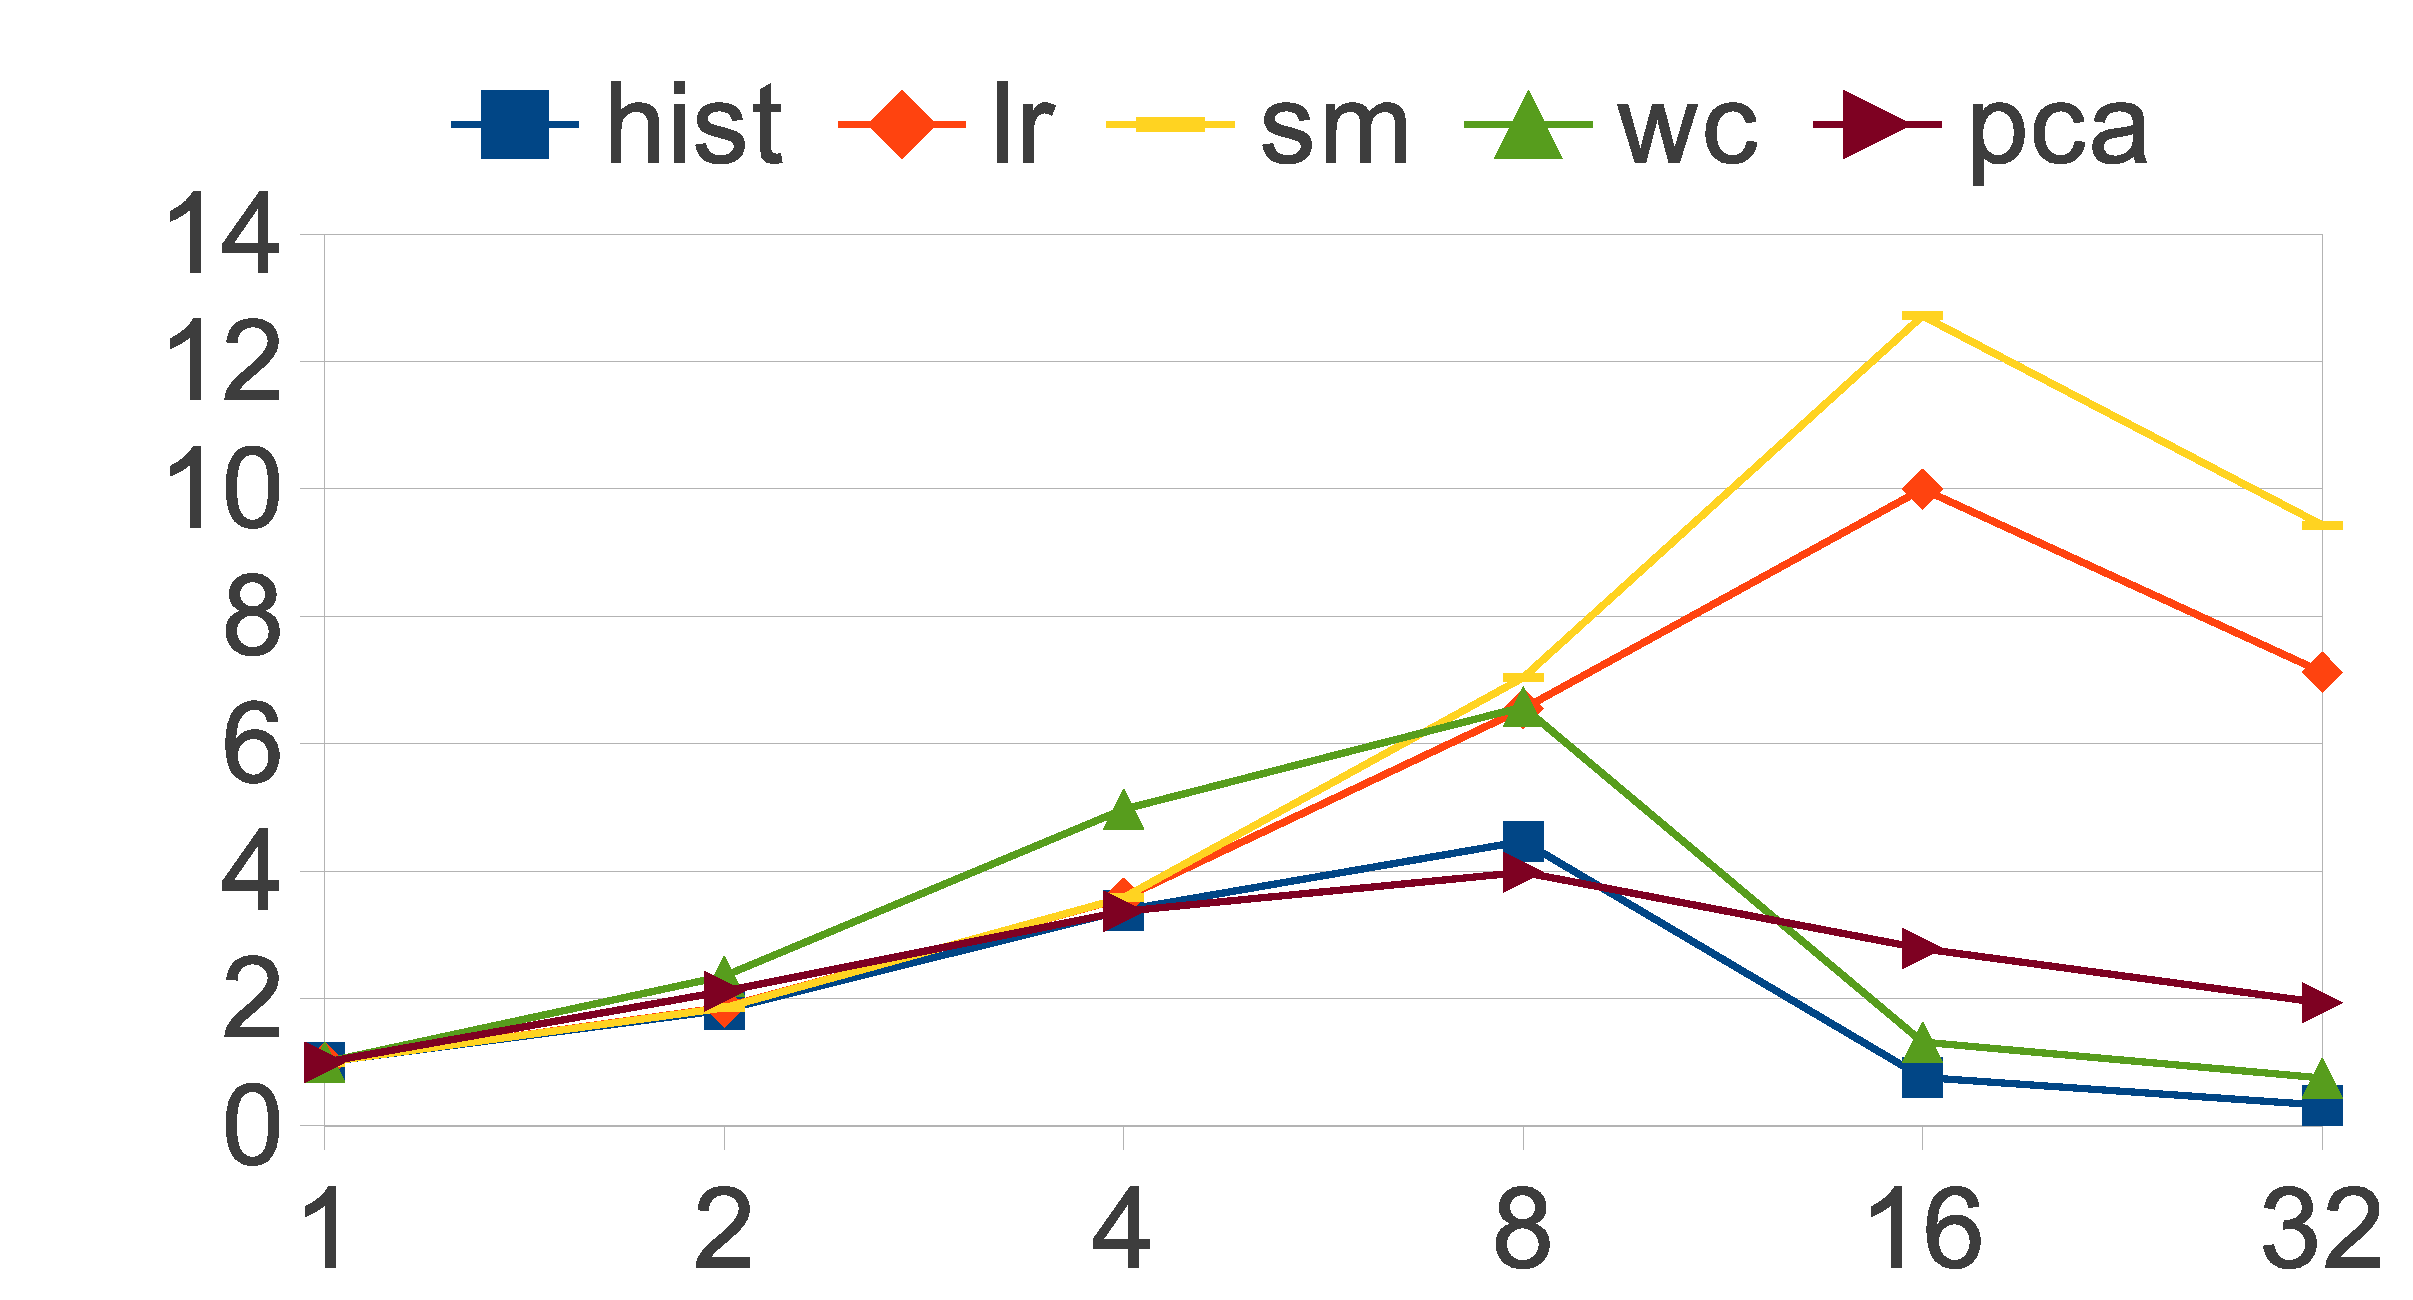
\includegraphics[width=0.5\textwidth]{img/phoenix_speedup.eps}
    \caption{Phoenix不开启Combiner情况下的Speedup}
    \label{phoenix:speedup}
\end{figure}
如图\ref{phoenix:speedup}的数据结果
(speedup计算方法为:高核下的运行时间/单核下的运行时间),
我们可以得出这样的结论:
随着核数的增多,4核以下,Phoenix的性能越来越好;
超过4核,Phoenix的性能却越来越差,特别是hist, wc, pca。

Phoenix的上述特性意味着,针对低核的机器,
它能够充分利用其资源,对于高核处理器,
Phoenix并不能充分利用资源。
Phoenix不适合在8核以上的机器上运行。
然而,多核机器是一个趋势,
一个CPU甚至达到上百的core\cite{Borkar2007Thousand},
随着多核机器上核数的不断增多,Phoenix便不具有实际的可用性。

制约Phoenix性能的主要因素有以下几点:
\begin{enumerate}
  \item Phoenix基于Posix线程库实现,开启的线程越多,
  需要共享的内核资源越多,会因为竞争这些资源
  以及共享的数据结构导致过高的spinlock.
  在32核情况下,hist的spinlock占用71.25\%。
  后续章节会详细分析Phoenix的spinlock问题。
  
  \item 由于中间结构的局限,
  Phoenix中Map阶段与Reduce阶段中间
  存在一个严格的barrier,降低了map和reduce线程
  并发的程度。此外,通常情况下,map是computation-intensivex的,
  reduce是memory-intensive的\cite{talbot2011phoenix++},
  barrier会导致资源的利用率比较低。
\end{enumerate}

DMR将针对上述的局限性进行改进和优化,
即避免Spinlock以获得较好的scalability,
同时打破原来的barrier,
增加Map和Reduce阶段并发的程度,
从而获得更好的性能。





  
